\documentclass[11pt]{article}

\usepackage{sectsty}
\usepackage{graphicx}
\usepackage{float}
\usepackage{wrapfig}
\usepackage{fancyhdr}
\usepackage{eso-pic}

\usepackage{listings}
\usepackage{color}

\graphicspath{ {./img/} }

\definecolor{dkgreen}{rgb}{0,0.6,0}
\definecolor{gray}{rgb}{0.5,0.5,0.5}
\definecolor{mauve}{rgb}{0.58,0,0.82}
\setcounter{section}{-1}
\lstset{frame=tb,
  language=Java,
  aboveskip=3mm,
  belowskip=3mm,
  showstringspaces=false,
  columns=flexible,
  basicstyle={\small\ttfamily},
  numbers=none,
  numberstyle=\tiny\color{gray},
  keywordstyle=\color{blue},
  commentstyle=\color{dkgreen},
  stringstyle=\color{mauve},
  breaklines=true,
  breakatwhitespace=true,
  tabsize=3
}

% Margins
\topmargin=-0.45in
\evensidemargin=0in
\oddsidemargin=0in
\textwidth=6.5in
\textheight=9.0in
\headsep=0.25in

% Template

\definecolor{greenIMT}{rgb}{0.6431,0.8235,0.2}

\pagestyle{fancy}
\fancyhf{}

\setlength{\headheight}{16pt}
\setlength{\footskip}{45pt}


\renewcommand{\headrule}{%
\vspace{-8pt}\hrulefill
\raisebox{-2.1pt}{}\hrulefill}

\fancyhead[L]{\nouppercase{\rightmark\hfill\leftmark}}
%\fancyhead[R]{\nouppercase{\leftmark\hfill\rightmark}}

\fancyfoot[L]{
    
\includegraphics[width=0.15\textwidth]{IMTAlogo.jpg}
}

\fancyfoot[C]{
    \thepage
}

\fancypagestyle{firstPage}{
    \fancyhf{}
    \fancyhead[R]{
        
\includegraphics[width=0.8\textwidth]{deco_cover_page.png}
    }
    \fancyfoot[L]{
        
\includegraphics[width=0.25\textwidth]{IMTAlogo.jpg}
    }
    
}
%SOLUTION : faire des minipages (2), 1 en bas et 1 en haut
%\renewcommand{\maketitle}{
	%\singlespacing
	%\thispagestyle{firstPage}
	%\renewcommand{\headrulewidth}{0pt}
	%\begin{flushleft}
	%\vspace*{320pt}
    %\begin{minipage}{20cm}
	\title{\textbf{\textcolor{greenIMT}{\Huge Rapport de suivi de projet}}}
    \author{{\Large SIT 213 -- Projet fil rouge} \\\\ FAVREL Antoine, RAVAUX Louis, Huguet Benjamin, Donatien Maëva}
    \date{\today}
    %\end{minipage}
    %\end{flushleft}
    %\vspace*{\fill} 
 %}   

\begin{document}
%\AddToShipoutPicture*{\BackgroundPic}

\maketitle
\pagebreak

% Optional TOC
\tableofcontents
\pagebreak
%--Paper--

\section{Le Projet}
\subsection{Objet du document}

Ce document a pour objectif le suivi du projet "Atelier logiciel - système de transmission"
Vous trouverez dans ce document l'ensemble des itérations, les tests réalisés, et les modifications apportées tout au long du projet.

\subsection{Cahier des charges}

L'objectif consiste à transmettre un message d'un point d'entrée à un point de sortie, via un canal de transmission (ou de communication). Le message d'entrée est émis par une source d'entrée. Les messages considérés dans ce projet seront des suites de symboles binaires (0 ou 1) correspondant à des informations échantillonnées et quantifiées sur deux niveaux logiques. Le message de sortie sera - autant que faire se peut - semblable au message d'entrée. Ce dernier étant incapable de traverser le canal de propagation tel quel, on l'adaptera aux caractéristiques physiques du canal en le convertissant au moyen d'un transducteur en un " vecteur " adapté à la transmission, appelé signal.

Ce dernier sera injecté dans le canal au moyen d'un émetteur. À l'autre extrémité du canal, il sera récupéré et traité par le récepteur et le transducteur de réception.

Les principaux canaux de transmission rencontrés dans la nature sont : le canal Hertzien (espace libre), le canal guidé électrique (câble), le canal guidé Optique (fibre), le canal acoustique aérien et le canal acoustique sous-marin. Chaque canal de propagation devant être utilisé à une fréquence bien particulière, le message est transposé autour de cette fréquence par l'opération de modulation. En outre, le canal sera une source de bruit pour les signaux qu'il transporte. Les principales sources de bruit rencontrées en pratique sont : la dispersion de trajets, la dispersion chromatique, le bruit de détection (grenaille), le bruit thermique et le bruit d'amplification.

Par la suite, chaque composant du système de transmission entre la source et la destination sera dénommé transmetteur.

\begin{figure}[H]
    \centering
    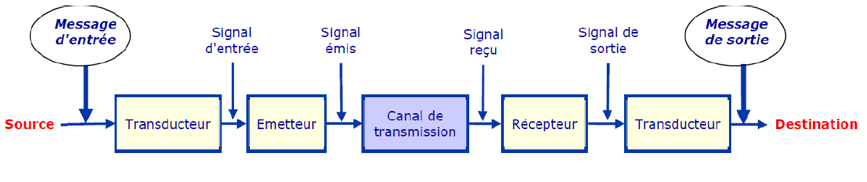
\includegraphics[width=1\textwidth]{image 1.png}
    \caption{\label{fig:image1}Composants de la chaine de transmission.}
\end{figure}

\pagebreak

\section{Iteration n°1}
\subsection{Objectifs}

L'objectif de cette première itération est avant tout de prendre en main la chaine de transmission.

Pour cette itération, la chaine respectera les propriétés suivantes :

La source émet une séquence booléenne soit fixée, soit aléatoire.
Le transmetteur logique parfait se contente, à la réception d'un signal, de l'émettre tel quel vers les destinations qui lui sont connectées.
La destination se contente de recevoir le signal du composant sur lequel elle est connectée.
Des sondes logiques permettent de visualiser les signaux émis par la source et le transmetteur parfait.
L'application principale calcule le taux d'erreur binaire (TEB) du système.

Voici un schéma de la chaine :

\begin{figure}[H]
    \centering
    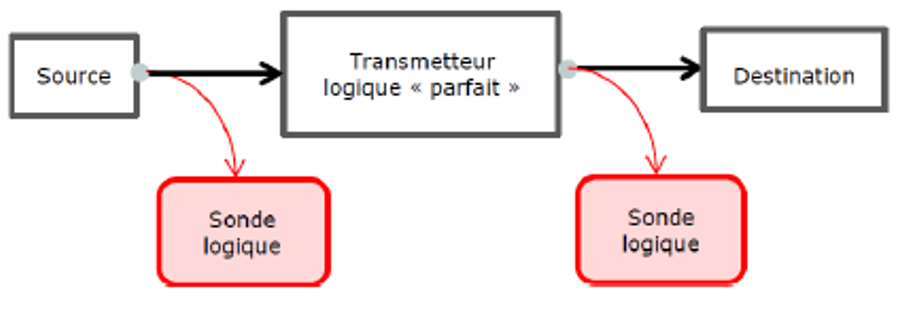
\includegraphics[width=1\textwidth]{image 2.png}
    \caption{\label{fig:image2}Chaine de transmission itération 1.}
\end{figure}

\subsection{Choix d'implémentation}

Pour permettre une utilisation simple et rapide du simulateur, la mise en place de scripts de compilation, de création de documentation et d'éxécution
ont été mis en place. Ces scripts sont disponibles à la racine du projet.
Il est donc possible de compiler puis tester le simulateur en utilisant les divers arguments spécifiés dans le readme.

Les différentes fonctionnalitées implémentées dans l'étape 1 (transmetteur parfait) sont les suivantes:
nbsample

En prévision d'une potentielle fusion de binômes, nous avons décidé de mettre en place une architecture logicielle versionné sur git.
Elle nous permettra à chacun de reprendre le projet et de travailler sur des fonctionnalitées différentes sans avoir à se soucier des conflits de version.

\subsection{Actions réalisées}

\subsubsection{Sources}

Dans un premier temps, nous avons créé deux classes sources. Une source fixe, qui envoie toujours la même séquence de données. Puis une source aléatoire qui envoie une nouvelle séquence à chaque appel.

\subsubsection{Transmetteur}

Par la suite, nous avons créé un transmetteur parfait. Il joue le rôle du canal de propagation. Pour ce transmetteur parfait, le canal transmet exactement ce qu'il reçoit.

\subsubsection{Destination}

Enfin, nous avons créé une destination. Cette classe joue le rôle de récepteur dans la chaine de transmission.

\subsection{Simulation}

Lors de l'execution de la commande: 

\begin{figure}[H]
    \centering
    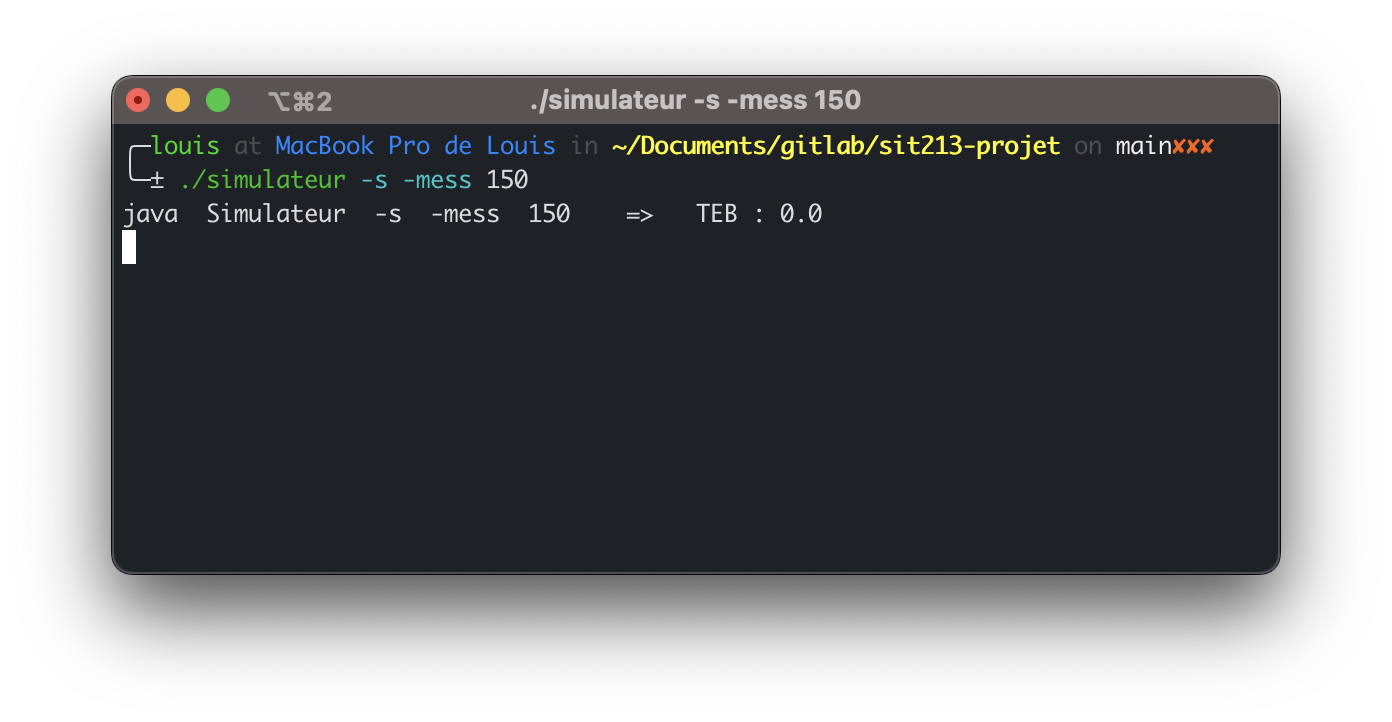
\includegraphics[width=\textwidth]{term_1.png}
    \caption{terminal}
\end{figure}

On constate lors de l'execution du script l'affichacge d'un signal identique sur la source et la destination (voir figure 2). Cela coincide 
avec le fait que le transmetteur est parfait et que le signal n'est donc pas modifié lors de la transmission vers la destination.
Le TEB est égal à 0 comme attendu.

\begin{figure}[H]
    \centering
    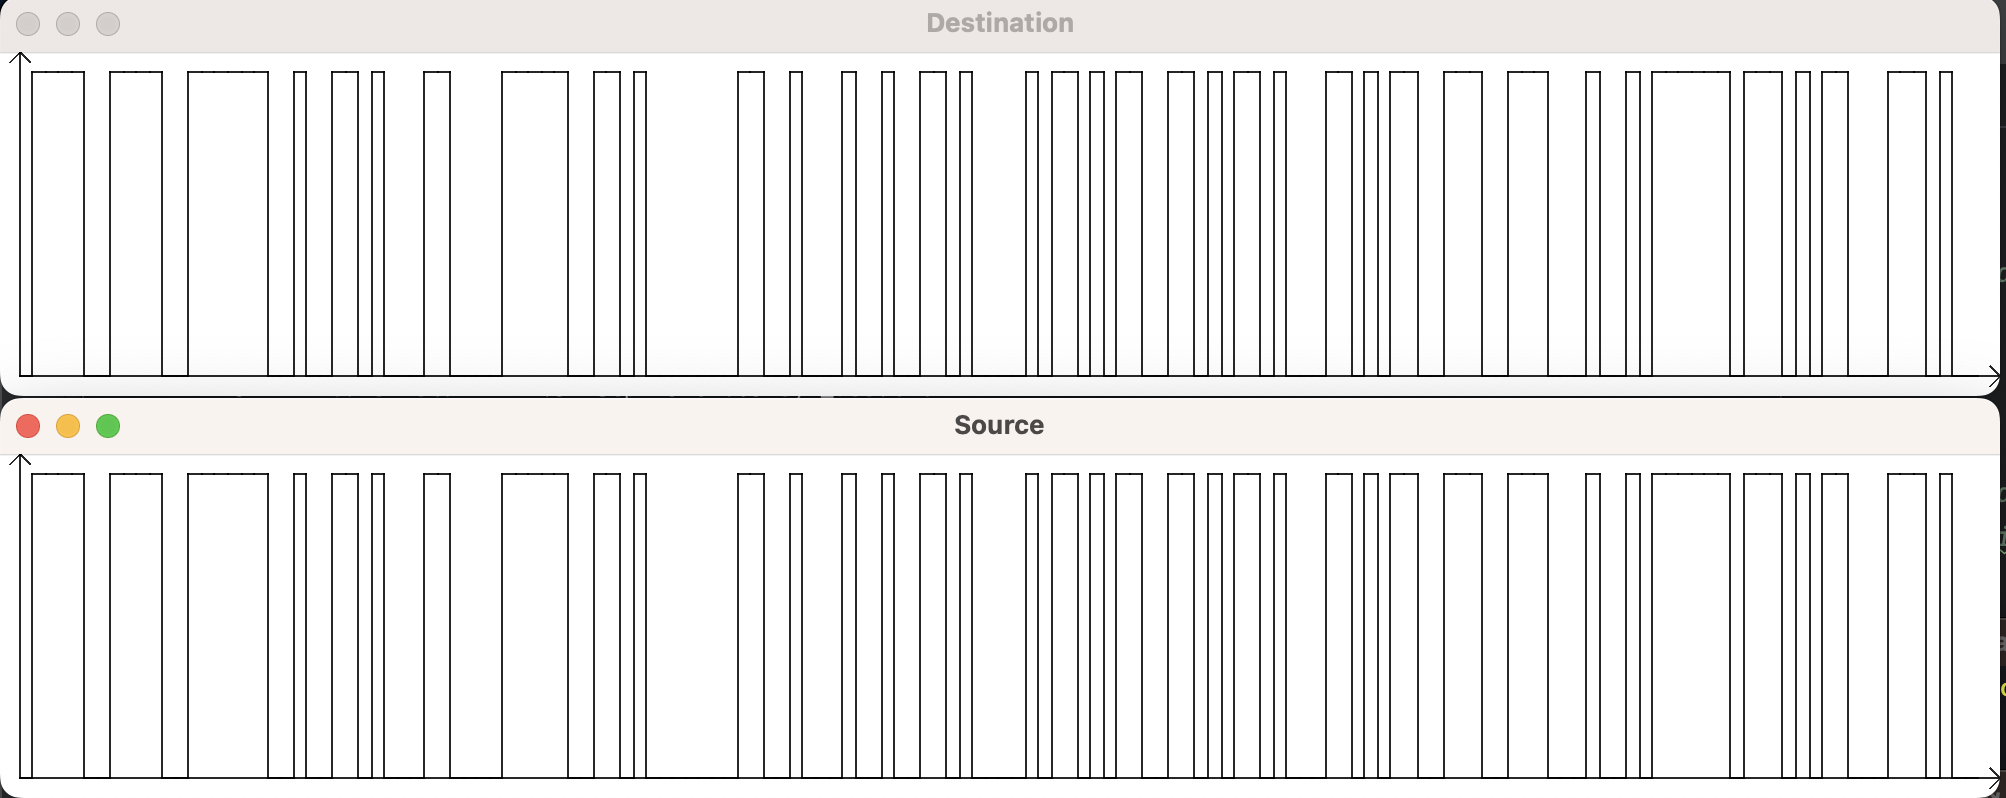
\includegraphics[width=\textwidth]{s_r_100.png}
    \caption{Execution du programme}
\end{figure}

\pagebreak

Executer le programme deux fois en utilisant la meme graine nous permet d'obtenir la meme génération de signal.
Cela nous sera utile dans le cadre de tests ultérieurs afin de s'assurer du bon fonctionnement du simulateur dans plusieurs situations différentes.

\begin{figure}[H]
    \centering
    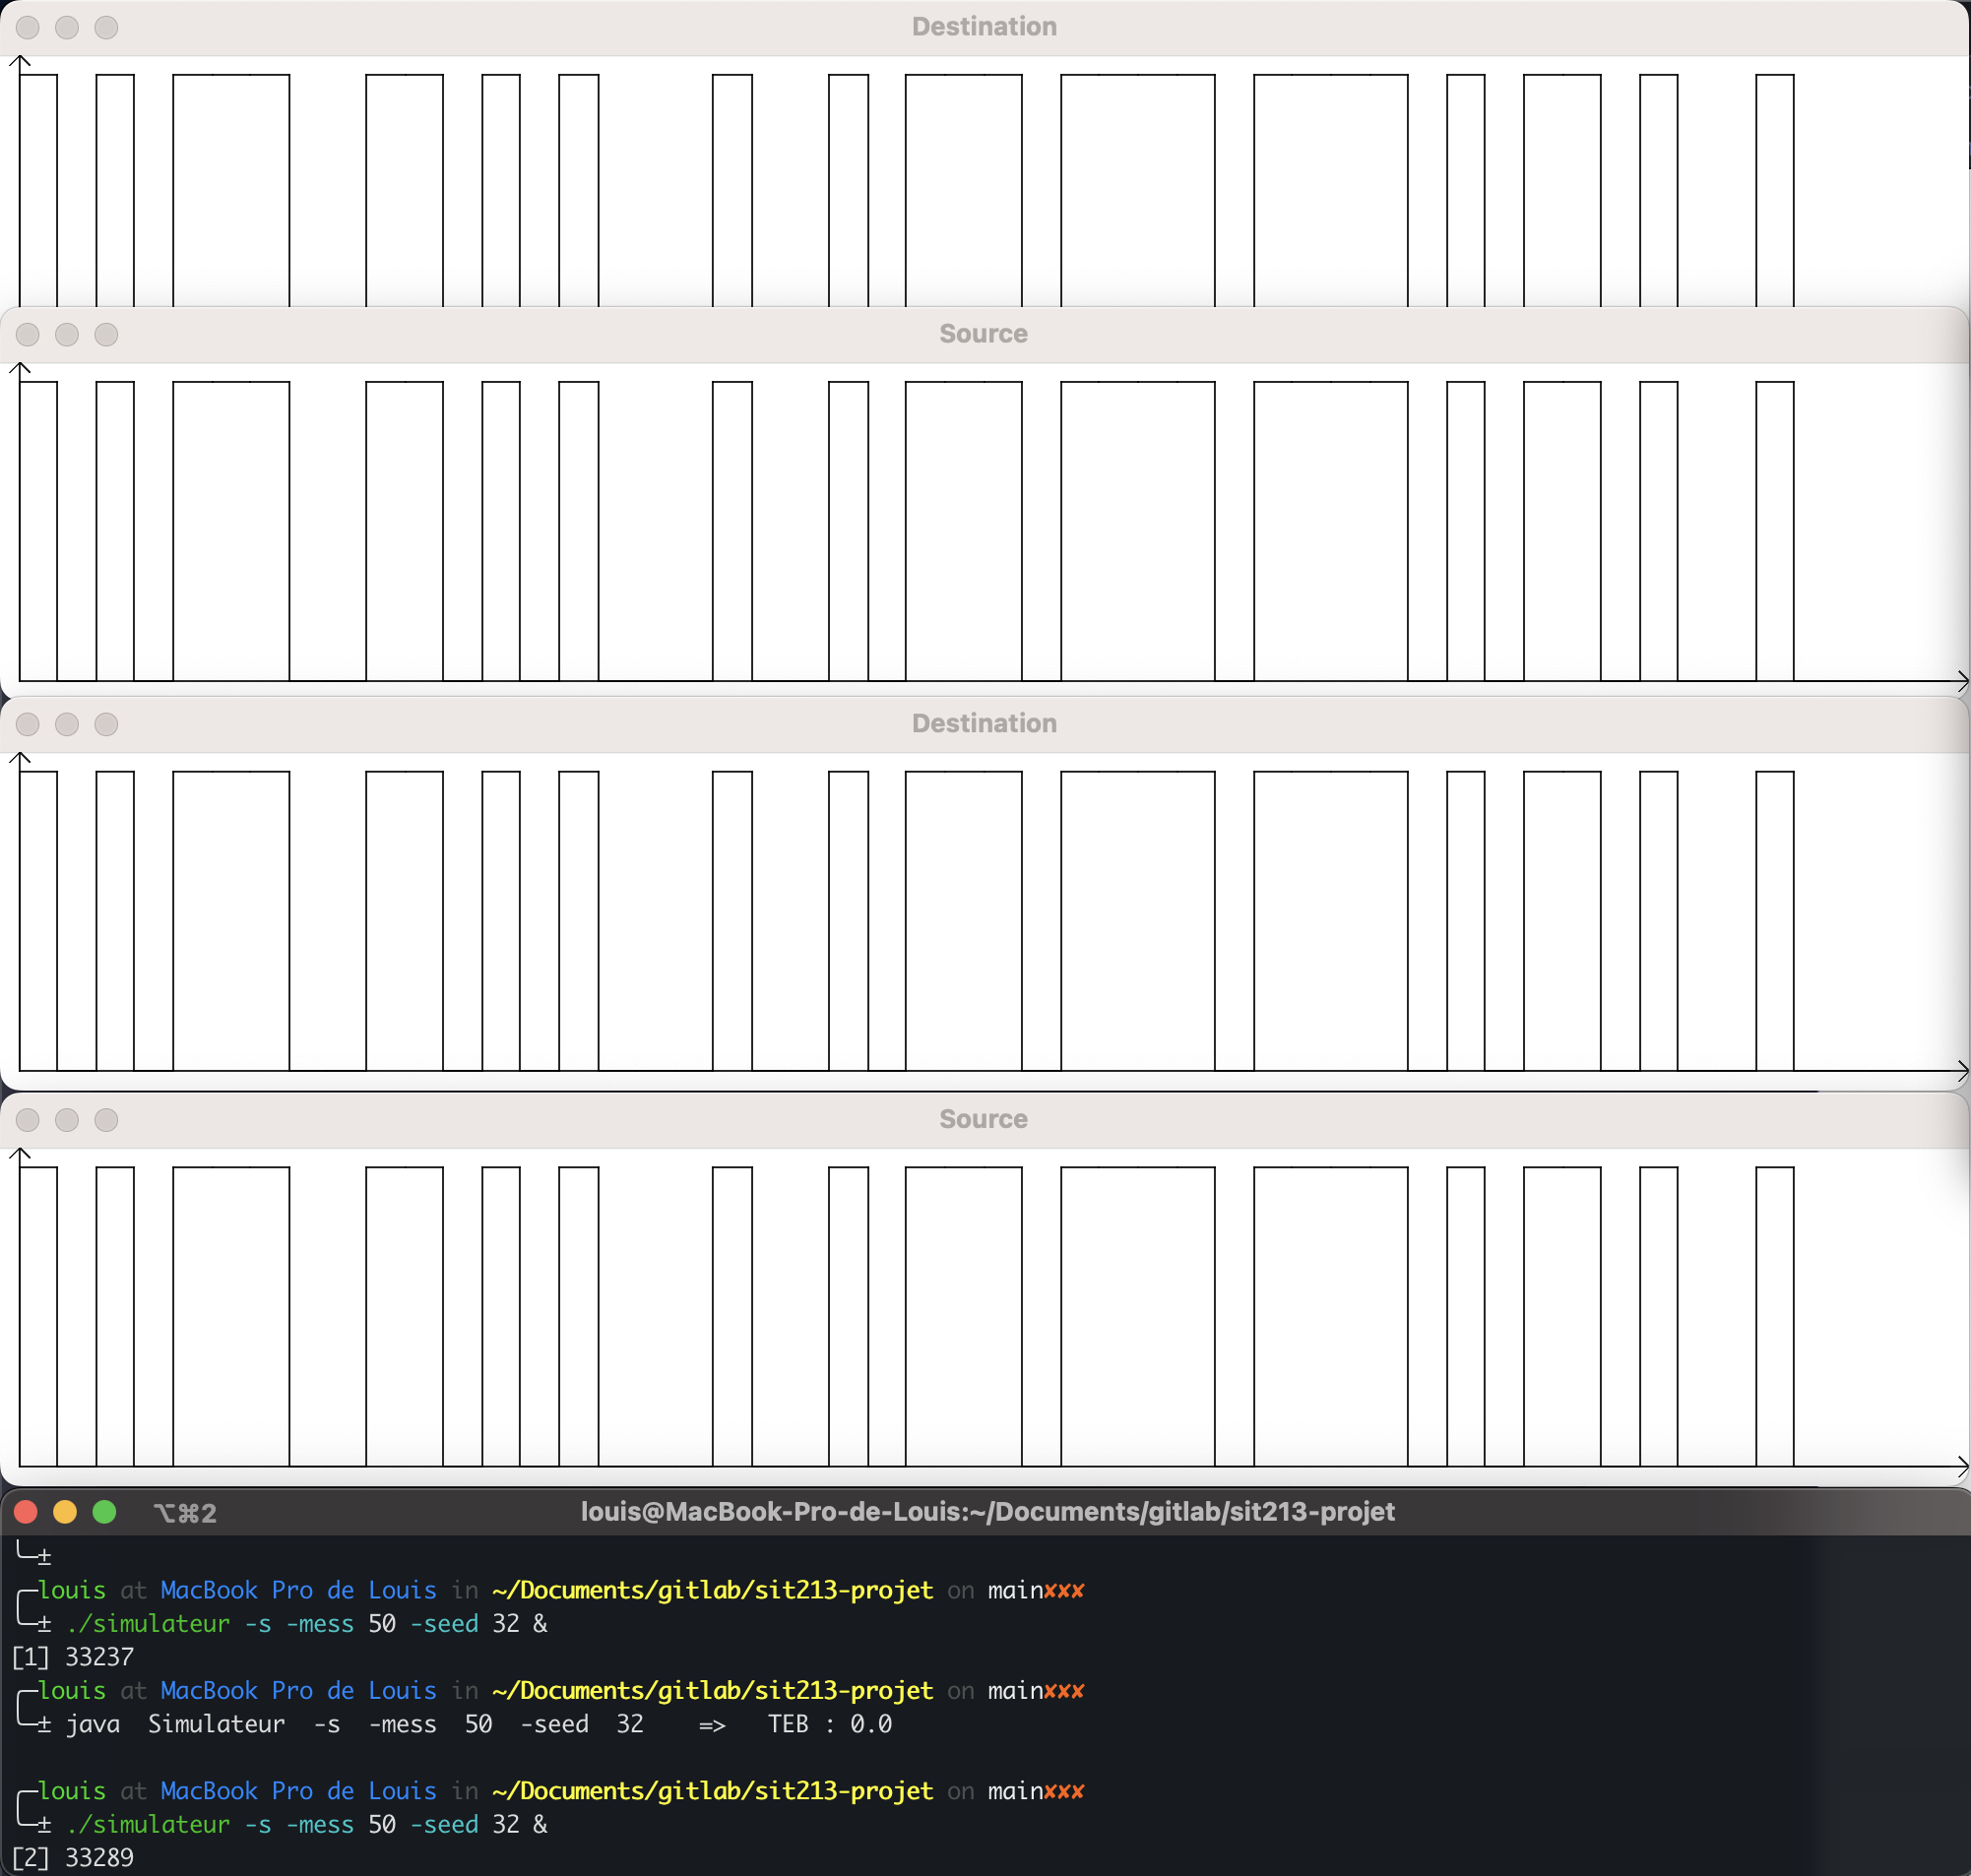
\includegraphics[width=\textwidth]{s_r_50.png}
    \caption{Exemple utilisation d'une "seed"}
\end{figure}

Nous observons que la sortie du transmetteur est purement identique à la source. C'est normal car il s'agit d'un canal parfait. Le TEB est donc de 0.

\subsection{Conclusion}

Cette première étape a été très utile dans la compréhension de l'architecture logicielle mise à disposition.
Cela aura été l'occasion de commencer à penser à l'organisation du travail d'équipe à venir et de mettre en place des outils de travail collaboratif.
Par ailleurs, notre chaine de transmission est fonctionnelle, nous sommes en mesure de choisir le type de source et observer la sortie du canal.
Pour le moment, nous n'avons qu'un seul type de transmetteur et que deux types de sources. Par la suite, nous serons amenés à mettre en œuvre une chaine de transmission avec des signaux analogiques et des canaux de propagations non-parfaits.
\pagebreak

\section{Itération n°2}
\subsection{Objectif de l'itération}

Dans cette nouvelle itération, nous allons devoir coder des émetteurs et un récepteur afin de convertir le signal logique en un signal "analogique" NRZ (non-retour à zéro), RZ (retour à zéro) et NRZT. Le rôle du récepteur sera de convertir n'importe quel signal analogique en un signal logique. Pour se faire, nous allons donc devoir modifier notre code afin de répondre aux exigences.

\begin{figure}[H]
    \centering
    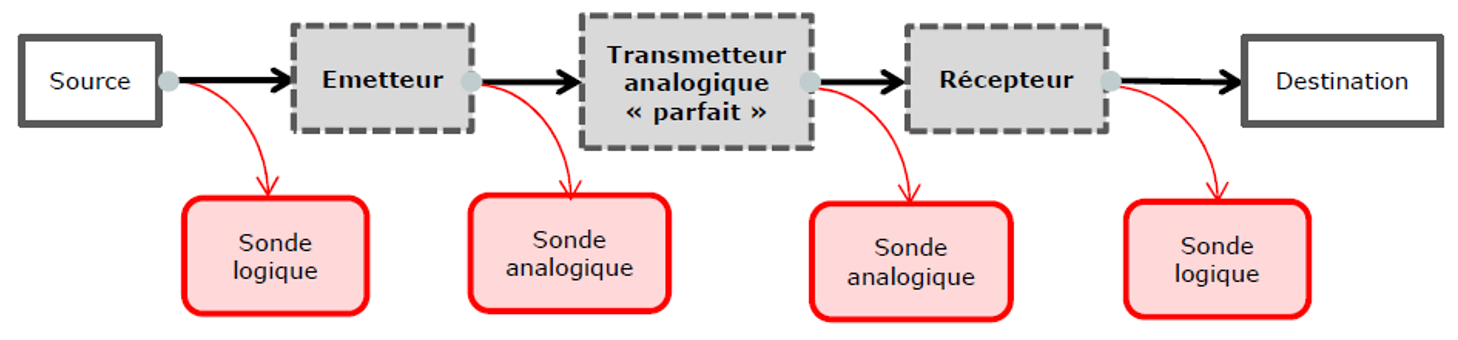
\includegraphics[width=1\textwidth]{image 5.png}
    \caption{\label{fig:image5}Chaîne de transmission itération n°2.}
\end{figure}

Un signal RZ signifie que le signal sera à l'état haut lorsque des 1 logiques seront transmis et à l'état bas lorsqu'il s'agit de 0 logique pendant la première demi-période. Il y a un retour à 0 à la deuxième demi-période du symbole (figure de gauche). Cependant dans ce projet, nous partirons du principe que l'émission à $V_{max}$ ou $V_{min}$ se situe entre le 1er et le 3ème tiers de la période symbole (figure de droite).

\begin{figure}[H]
    \centering
    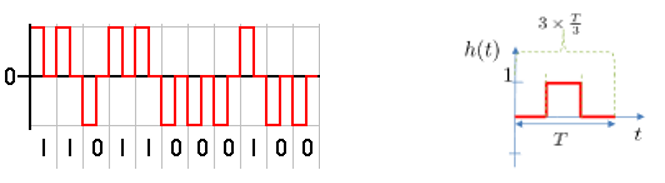
\includegraphics[width=1\textwidth]{image 6.png}
    \caption{\label{fig:image6}Schémas explicatifs signal RZ.}
\end{figure}

Un signal NRZ signifie que le signal sera à l'état haut lorsque des 1 logiques seront transmis et à l'état bas lorsqu'il s'agit de 0 logique. Contrairement au RZ, l'état est le même pendant toute la durée du temps symbole et d'utiliser trois fois moins de bande passante dans notre cas.

\begin{figure}[H]
    \centering
    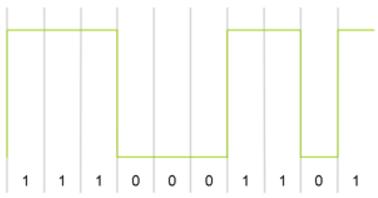
\includegraphics[width=0.5\textwidth]{image 7.png}
    \caption{\label{fig:image7}Schéma explicatif signal NRZ.}
\end{figure}

Un signal NRZT possède les mêmes propriétés qu'un signal NRZ. Cependant pour simuler le temps de montés des composants, chaque changement d'état sera représenté par une monté et descente progressive symbolisé sur $\frac{1}{3}$ des périodes symboles.

\begin{figure}[H]
    \centering
    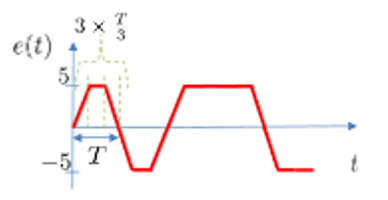
\includegraphics[width=0.5\textwidth]{image 8.png}
    \caption{\label{fig:image8}Schéma explicatif signal NRZT.}
\end{figure}

\textcolor{red}{Le cahier des charges nous donne des amplitudes maximum et minimum à respecter. Pour le codage NZR et NRZT, il faut que $V_{max} >= 0$ et $V_{min} >= 0$ et $V_{max} > V_{min} $
Pour le signal RZ, il faut que $V_{max} >= 0$ et $V_{min} = 0$ et $V_{max} > V_{min} $ }

\subsection{Organisation}

Pour nous permettre de répondre aux demandes de l'itération (mise en place d'une transmission analogique), nous allons devoir créer deux nouveaux éléments par rapport au code de la première itération. Ces modifications devront nous aider à lancer le programme tout en prenant en compte les paramètres d'entrée que nous rentrerons dans le terminal.
Nous ne devrions plus avoir d'erreurs sur notre code et ne pas avoir d'erreurs sur les signaux émis et reçus. Pour vérifier cela, nous utiliserons le calcul du TEB et afficherons les graphiques permettant de comparer à vue d'œil les éventuelles erreurs et leur emplacement.
Avant de commencer à développer notre code nous avons utilisé l'application "Project" d'Office 365 afin de nous permettre de créer un diagramme de Gant. Ce diagramme nous permet de classer les actions à faire (par catégories, par acteurs, par priorité) et de mettre des échéances afin de respecter les délais. Vous trouverez ci-dessous un exemple de diagramme Gant que nous avons fait pour cette seconde itération :

\begin{figure}[H]
    \centering
    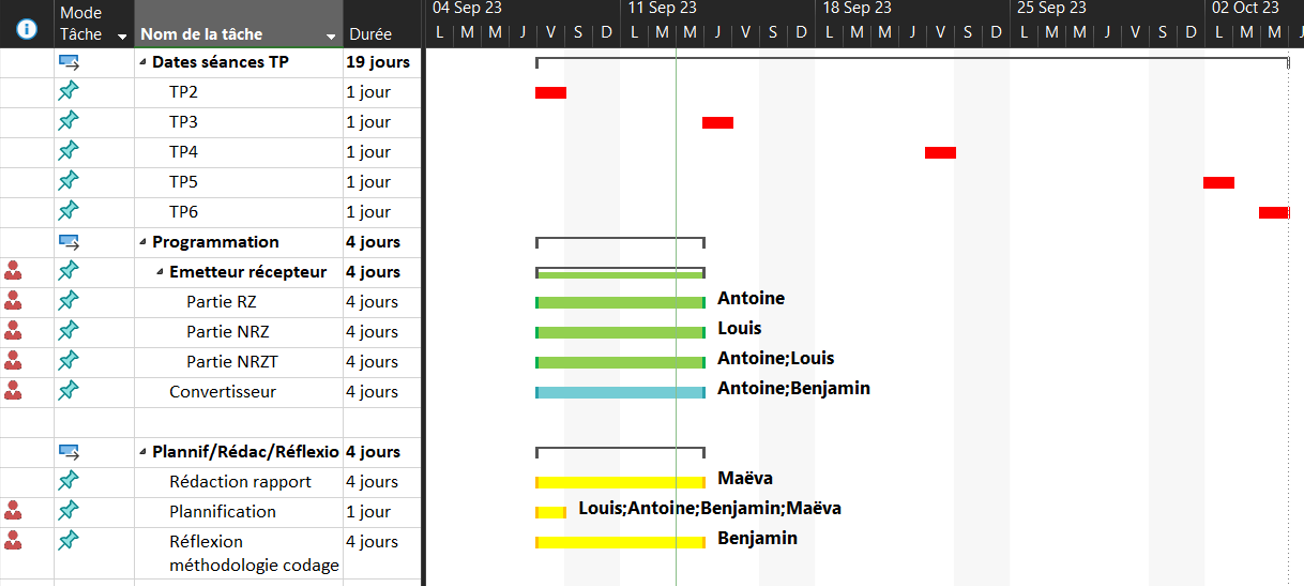
\includegraphics[width=1\textwidth]{image 9.png}
    \caption{\label{fig:image9}Diagramme de Gant itération 2.}
\end{figure}

Pour le développement de notre code, nous allons utiliser l'application Intellij Idea nous permettant de partager plus facilement les codes que nous déposons sur le projet que nous avons créé sur GitLab. La combinaison des 2 nous permet de modifier le code tous en même temps sans empiéter sur les modifications des-uns et des-autres. Intellij Idea nous permet également de créer des branches et de ne commit sur une interface graphique. Il est donc important de se répartir les tâches, ce que nous avons fait dans le diagramme de Gant.

\subsection{Procédures de développement}
\subsubsection{Emetteur}

L'émetteur à un rôle important. Il permet de convertir un signal logique en signal pseudo-analogique. Trois codages en ligne sont attendus pour ce projet. La logique qui repose sur ceux-ci sont la même. On prend le signal logique en entrée, puis en fonction de son état (0 ou 1), on le transforme en une série de flottant qui sera adapté au codage en ligne souhaité. Le nombre d'échantillonnage par symbole sera un paramètre à choisir lors des lancements de simulations (nommé nb\_samples par la suite) ainsi que l'amplitude maximum ($V_{max}$) et minimum ($V_{min}$).

\textbf{Emetteur NRZ :}

Il s'agit de l'émetteur le plus simple à coder. On prend le symbole logique en entrée et s'il s'agit d'un état à 1, alors on émet un nombre de flottant égale à nb\_samples ayant pour amplitude $V_max$. Pour l'état à 0, on émet le même nombre de flottant mais ayant pour amplitude $V_{min}$.

\begin{figure}[H]
    \centering
    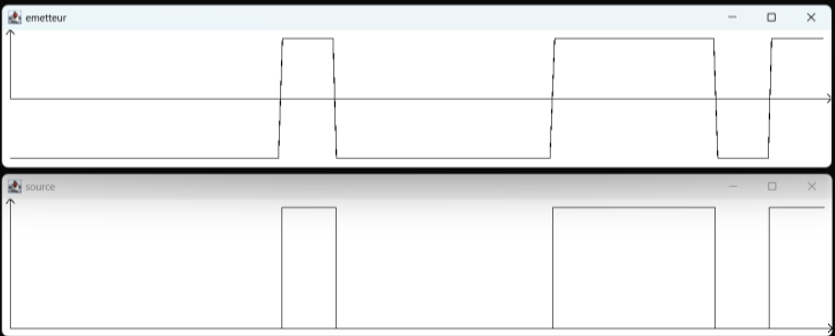
\includegraphics[width=1\textwidth]{image 10.png}
    \caption{\label{fig:image10}Sortie de la source et de l'émetteur NRZ.}
\end{figure}

Ci-dessus le graphique en sortie de la source et de l'émetteur NRZ. On retrouve bien une amplitude égale à $V_{max}$ pendant une durée symbole pour un état logique 1 et une amplitude égale à $V_{min}$ pendant une durée symbole pour un état logique à 0.

Emetteur RZ :

L'émetteur RZ est légèrement plus compliqué que le signal NRZ. La construction d'un symbole se passe en trois étapes.

\begin{itemize}
    \item Sur le premier tiers $(\frac{nb\_samples}{3})$, les flottants ont pour amplitude 0.
    \item Sur le deuxième tiers $(]\frac{nb\_samples}{3}$,$\frac{nb\_samples}{3}*2])$, les flottants ont pour valeur $V_{max}$ si le bit d'état logique est à 1 et $V_{min}$ si le bit est à 0.
    \item Sur ce dernier tiers, les flottants ont de nouveau une amplitude de 0.
\end{itemize}

\begin{figure}[H]
    \centering
    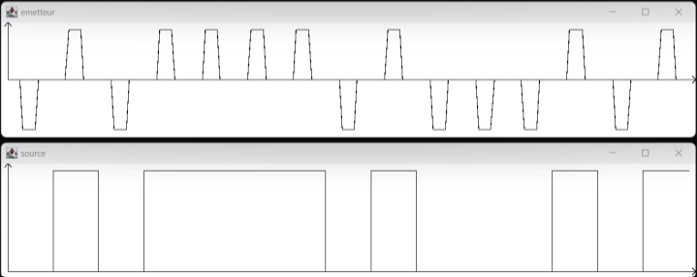
\includegraphics[width=1\textwidth]{image 11.png}
    \caption{\label{fig:image11}Sortie de la source et de l'émetteur RZ.}
\end{figure}

Ci-dessus le graphique en sortie de la source et de l'émetteur RZ. On apercevoir qu'un symbole logique est représenté par un symbole analogique composé en trois parties : le premier et dernier tiers à 0 et le deuxième tiers avec une amplitude à $V_{max}$ ou $V_{min}$.

\textbf{Emetteur NRZT :}

C'est le transmetteur le plus complexe à faire. Il reprend les caractéristiques du NRZ mais possède une pente montante et descendante au 1er et dernier tiers. Avant toute chose, il faut calculer un pas qui sera utilisé pour la pente. Pour cela, on utilise cette formule : $ pas = \frac{Vx}{\frac{nb\_samples}{3}} $ avec $V_x$ ayant $V_{max}$ ou $V_{min}$ en fonction du bit logique.

La construction d'un sylmbole se passe en trois étapes :
\begin{itemize}
    \item Sur le premier tiers $ \left(\frac{nb\_samples}{3} \right) $, les flottants ont une amplitude déterminée par le pas pour construire une rampe vers $V_x$.
    \item Sur le deuxième tiers $(]\frac{nb\_samples}{3}, \frac{nb\_samples}{3}*2]) $, les flottants ont pour valeur $V_{max}$ si le bit d'état logique est à 1 et $V_{min}$ si le bit est à 0.
    \item Sur le dernier tiers, les flottants ont une amplitude déterminée par le pas pour construire une rampe vers 0. Néanmoins, si plusieurs bits logiques de même signe se suivent, il n'y a pas de rampe entre le premier et le dernier tiers des bits analogiques correspondants. On reste sur une amplitude $V_{max}$ et $V_{min}$.
\end{itemize}

\begin{figure}[H]
    \centering
    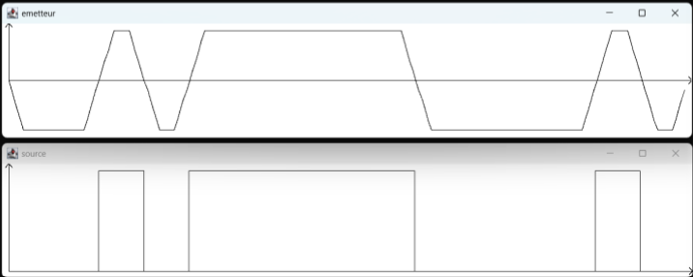
\includegraphics[width=1\textwidth]{image 12.png}
    \caption{\label{fig:image12}Sortie de la source et de l'émetteur NRZT.}
\end{figure}

Ci-dessus le graphique en sortie de la source et de l'émetteur NRZT. On remarque que le signal en sortie d'émetteur correspond bien à la description faite précédemment. On observe bien les pentes vers $V_x$ et 0 mais également la conservation de l'amplitude $V_x$ lorsque plusieurs bits logiques se suivent.

\subsubsection{Récepteur}

Le récepteur à un enjeu primordial, il est capable de recevoir un signal analogique et de le convertir en un signal logique (même type que le signal source). Notre exigence était d'avoir un seul récepteur qui puisse traiter n'importe quel signal analogique.
Pour ce faire, on utilise comme méthode de moyenner les valeurs reçues sur la durée d'un temps symbole. Préalablement, nous avons déterminer un seuil de décision qui correspond à $\frac{V_{max} + V_{min}}{2}$.
Il peut ainsi fluctuer en fonction des valeurs seuil choisi. Si la moyenne se situe au-dessus du seuil de décision, alors le bit d'état logique sera à 1. Si la moyenne se situe en-dessous du seuil de décision, alors le bit d'état logique sera à 0.

\subsection{Tests}

Par manque de temps, nous n'avons pas réalisé de test à proprement parler pour tester chaque ligne des nouvelles classes de l'itération. Nous avons seulement effectué un contrôle visuel grâce aux sondes placées aux différents endroits. Le principal contrôle étant de s'assurer que le signal reçu est le même que le signal émis comme il s'agit d'un canal parfait.
Pour les prochaines itérations, nous effectuerons de vrai test avec notamment des outils pour tester la couverture de ceux-ci.

\subsection{Performances}

Nous sommes toujours dans le cas d'un canal de transmission parfait. Que ce soit avec n'importe quel codage de signal, nous arrivons à retrouver les bits émis par la source.

Voici la simulation pour un signal généré grâce à une source aléatoire puis encodé en NRZ :

\begin{figure}[H]
    \centering
    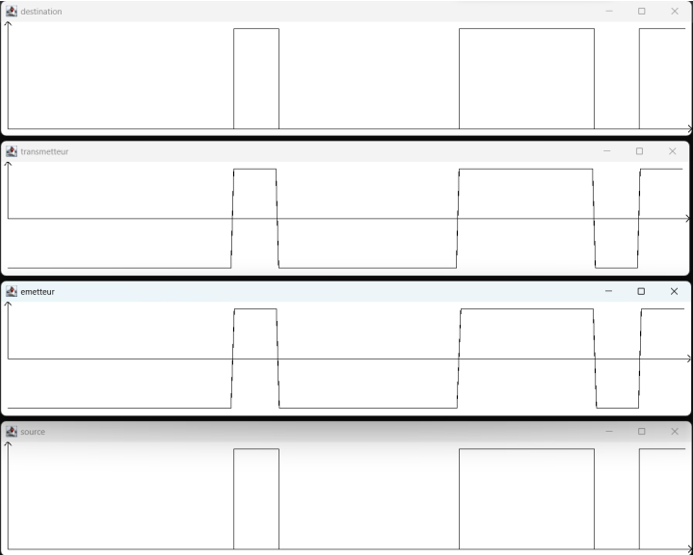
\includegraphics[width=1\textwidth]{image 13.png}
    \caption{\label{fig:image13}Simulation d'un signal généré puis encodé en NRZ.}
\end{figure}

Voici la simulation pour un signal généré grâce à une source aléatoire puis encodé en RZ :

\begin{figure}[H]
    \centering
    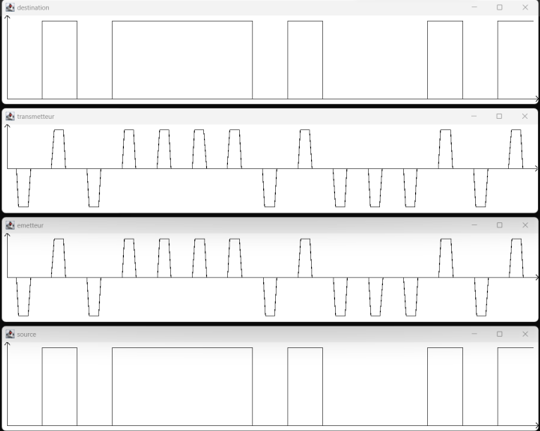
\includegraphics[width=1\textwidth]{image 14.png}
    \caption{\label{fig:image14}Simulation d'un signal généré puis encodé en RZ.}
\end{figure}

Voici la simulation pour un signal généré grâce à une source aléatoire puis encodé en NRZT :

\begin{figure}[H]
    \centering
    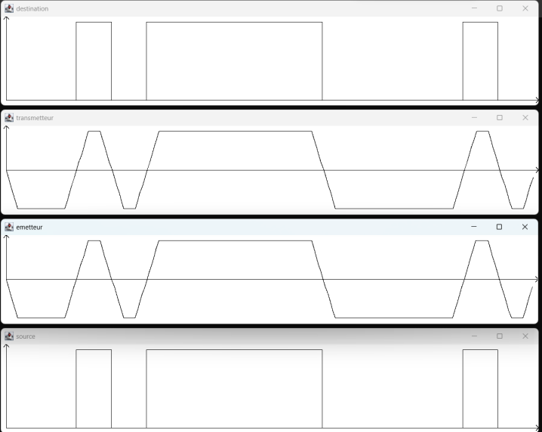
\includegraphics[width=1\textwidth]{image 15.png}
    \caption{\label{fig:image15}Simulation d'un signal généré puis encodé en NRZT.}
\end{figure}

Nous observons que la sortie du transmetteur est purement identique à la source. C'est normal car il s'agit d'un canal parfait. Le TEB est donc de 0. Le codage en ligne, quel qui soit, n'a pas d'impact
lorsqu'il est émis sur un transmetteur parfait.

\subsection{Conclusion}

Notre projet évolue. Lors de la première itération, notre chaine de transmission était opérationnelle avec comme fonctionnalités le type de source et l'observation de la sortie du canal.
Maintenant, nous sommes capables de convertir le signal de la source en un codage en ligne (RZ,NRZ et NRZT) et d'effectuer la manœuvre inverse en bout de canal afin de retrouver le signal de départ.

Nous avons également eu un problème de gestion du temps (mauvaise compréhension de la date de dépôt). Cette erreur ne nous a pas permis de livrer l'itération avec l'ensemble des attentes (tests, scripts). Ce manque sera comblé lors de la prochaine itération.
\textcolor{red}{Suite aux complications que nous avions eu lors de la seconde itération, nous avons profité de la troisième pour corriger nos erreurs et mettre à jour le code. Nous avons donc modifié le code du côté de l'emetteur pour le RZ afin que ce dernier fonctionne. Nous avons également modifié les codes du côté de l'émetteur et du récepteur pour le NRZT. Grâce à ces modifications nous n'avons plus de décalage lors de la simulation des signaux RZ et NRZT.}

Lors de la prochaine étape, il faudra créer un nouveau transmetteur afin d'avoir une transmission non-idéale avec canal bruité de type "gaussien".
\pagebreak

\section{Itération n°3}

\subsection{Objectif de l'itération}

Dans cette nouvelle itération, nous allons devoir modifier notre code afin que ce dernier puisse générer du bruit et gérer les problèmes au niveau du bruit et de sa puissance. Nous allons devoir coder une nouvelle classe afin qu'elle émette un bruit gaussien. Par ailleurs, nous devrons mettre en place un code nous permettant d'échantiller les signaux bruités reçu afin qu'ils correspondent aux signaux émis.

Ci-dessous le schéma correspondant à l'itération n°3.

\begin{figure}[H]
\centering
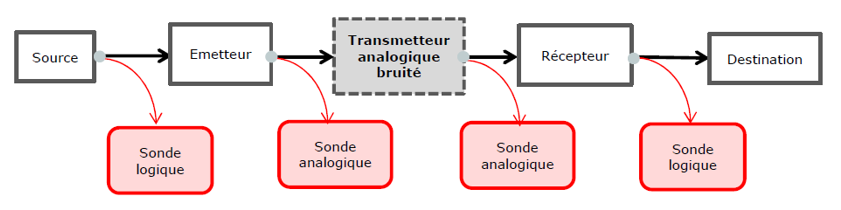
\includegraphics[width=1\textwidth]{image 16.png}
\caption{\label{fig:image16}Schéma de l'itération n°3.}
\end{figure}

Ci-dessous le schéma correspondant à l'ajout de bruit pour cette itération

\begin{figure}[H]
\centering
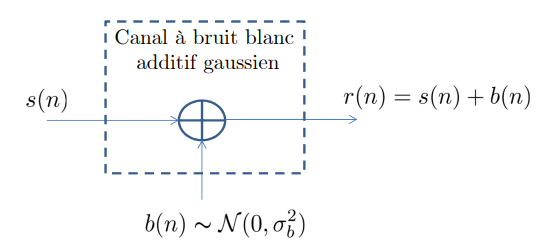
\includegraphics[width=0.8\textwidth]{image 17.png}
\caption{\label{fig:image17}Schéma d'ajout de bruit itération n°3.}
\end{figure}

Dans cette partie on nous demande également un graphique représentant le taux d'erreur binaire (TEB) en fonction du rapport signal sur bruit (SNR) par bit. Nous devons donc faire des modifications dans notre code afin de calculer le SNR et de modéliser la courbe.

\subsection{Organisation}

Pour nous permettre de répondre aux demandes de l'itération (mise en place de l'ajout d'un bruit blanc gaussien), nous allons devoir créer de nouveaux éléments par rapport au code de l'itération précédente. Ces modifications devront nous aider à lancer le programme tout en prenant en compte le bruit qui pourrait se trouver dans un canal de transmission. Nous ne devrions pas avoir d'erreurs sur notre code cependant nous devrions pouvoir observer l'ajout de bruit que nous avons effectué sur nos graphiques lors de la modélisation de notre signal transmis à la destination. Afin de vérifier le bon fonctionnement de notre code nous nous appuirons sur ces graphiques mais également sur les calculs du TEB, du SNR ainsi que sur la courbe TEB vs SNR.
En vue des modifications à effectuer, nous avons développé le diagramme de Gant que nous avions utilisé lors de la première itération afin d'affecter à chacuns des tâches pour permettre de pouvoir livrer l'itération à l'heure. Vous trouverez ci-dessous le diagramme de Gant pour cette troisième itération :

\begin{figure}[H]
\centering
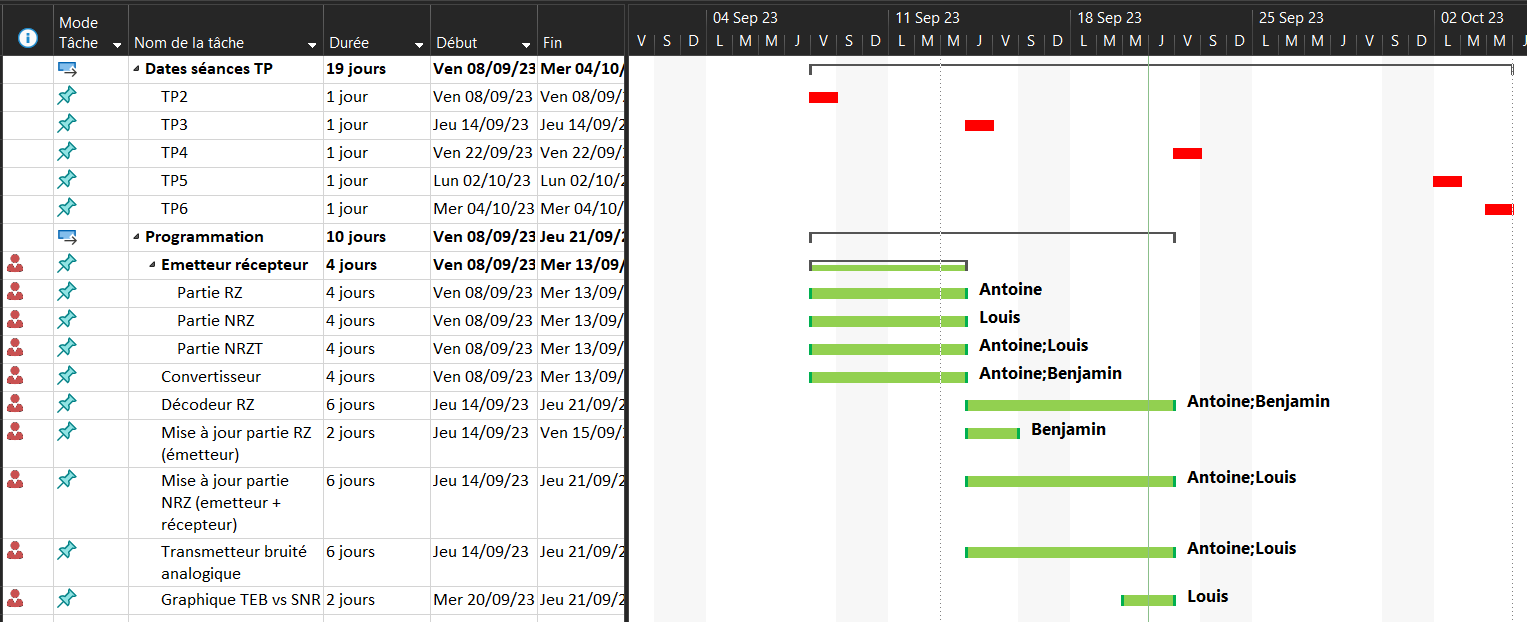
\includegraphics[width=1\textwidth]{image 18.png}
\caption{\label{fig:image18}Diagramme de Gant itération 3 (1/2).}
\end{figure}
\begin{figure}[H]
\centering
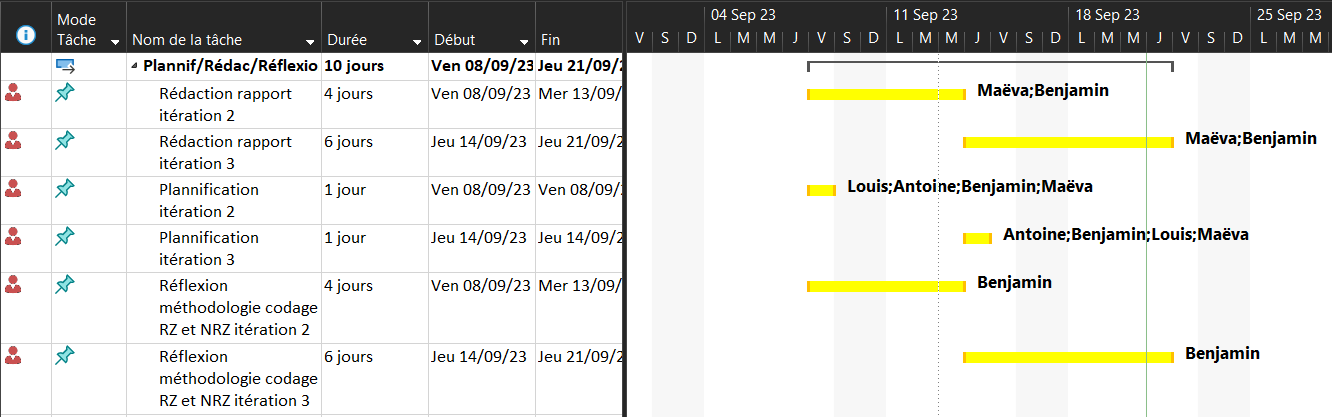
\includegraphics[width=1\textwidth]{image 20.png}
\caption{\label{fig:image20}Diagramme de Gant itération 3 (2/2).}
\end{figure}

Pour le développement de notre code nous avons utilisé l'application de bureau Intellij Idea, comme évoqué pour la seconde itération. Nous utiliserons cette application tout au long du TP. Nous avons également utilisé GitLab nous permettant de stocker le projet. Nous l'utiliserons également tout du long du TP.

\subsection{Procédures de développement}

Afin de répondre aux exigences de l'itération nous avons créé une nouvelle classe de type de composant transmetteur qui se nomme TransmetteurBruiteAnalogique. Le transmetteur est un élément clé dans une chaîne de transmission. Dans notre cas, ce dernier est analogique et nous permet donc de transmettre un signal analogique à partir d'informations numériques faites à base de 0 et de 1.

Dans cette itération, nous nous intéressons à la modulation du bruit et de son ajout au code et au signal final. Afin de modéliser ce bruit nous avons besoin de formules mathématiques que nous pouvons retrouver par raisonnement.

\subsubsection{Modélisation du bruit}
Pour la création de notre bruit nous utilisons la formule suivante :
$b(n) = \sigma_b\sqrt{-2*ln(1-a_1 (n))}cos(2\pi*a_2 (n))$ avec $a_1 (n) ~ \mathcal{U}[0,1[$ (loi uniforme) et $a_2 (n) ~ \mathcal{U}[0,1[$

Pour l'utiliser, il faut calculer la variance.
$\sigma = \sqrt{\frac{P_s*N}{2*10^{\frac{SNR}{10}}}}$
On remarque que notre bruit est généré en fonction de notre SNR.

Il nous reste plus qu'à injecter dans notre signal analogique le bruit généré précédemment. Ainsi, nous arrivons à simuler un signal bruité comme similaire dans la vraie vie à son arrivée dans le récepteur. Grâce à celui-ci, nous allons pouvoir tester la performance de nos codages de ligne.

\subsection{Performances}

Pour tester la perormance de ce système, on va générer deux fonctions permettant de vérifier deux paramètres différents.

\subsubsection{Graphe gaussien du bruit}

Lors de cette itération, nous avons utilisé la formule de Rice pour générer le bruit que l'on va additionner dans notre canal. Pour vérifier que notre bruit est bien blanc et gaussien, nous allons  dessiner un graphique qui va avoir comme données la puissance de bruit par rapport au nombre d'occurrence (voir le graphique ci-dessous).

\begin{figure}[H]
\centering
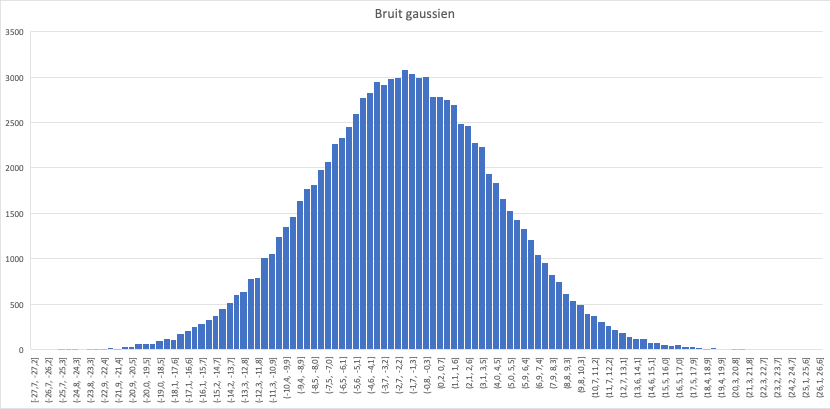
\includegraphics[width=1\textwidth]{img/gaussienne.png}
\caption{\label{fig:gaussienne}Gaussienne}
\end{figure}

\subsubsection{Test de la performance des codages de canal}

La deuxième série de valeur à générer permet de savoir à quelle SNR notre codage de ligne est considéré comme fiable.
Pour ce faire, on va tracer un graphique représentant le TEB en fonction du $\frac{RSB}{bit}$.

\begin{figure}[H]
\centering
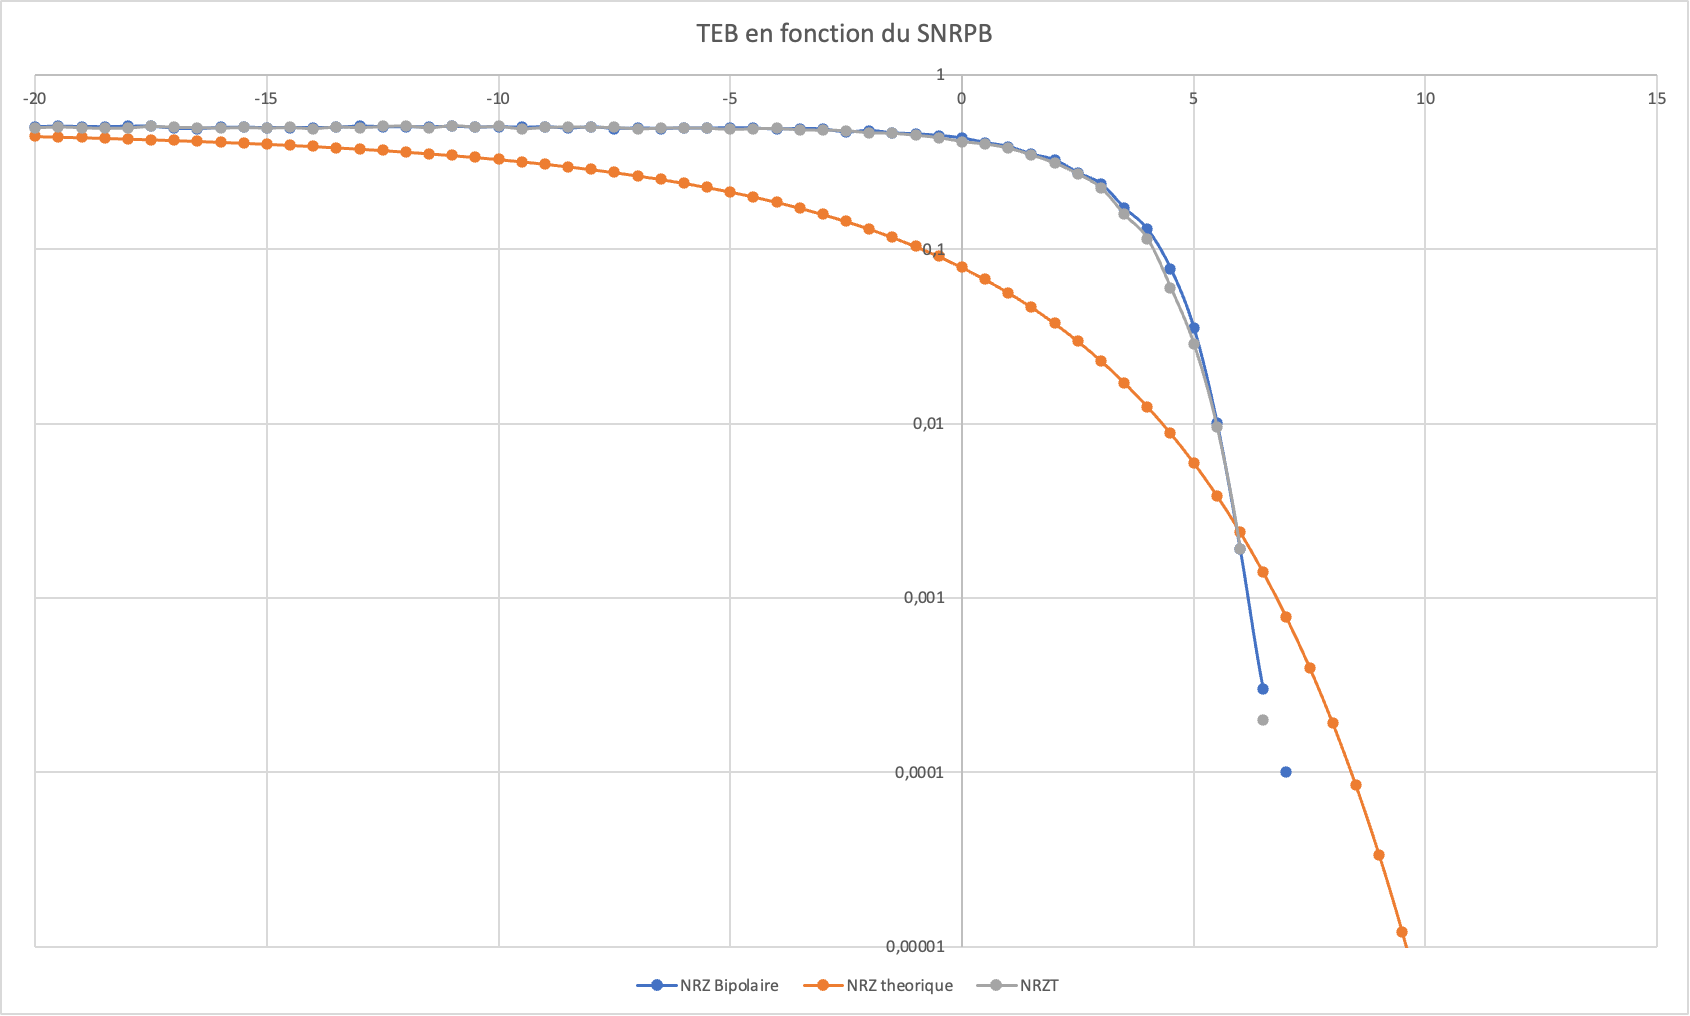
\includegraphics[width=0.9\textwidth]{img/tebvssnrpb.png}
\caption{\label{fig:TEBenFonctionDesSNR}Graphique du TEB en fonction du SNRPB.}
\end{figure}

\textcolor{red}{Après correction de notre calcul du bruit blanc gaussien, nous trouvons désormais des valeurs plus proche de la réalité. La courbe orange représente le TEB théorique du NRZ. Nous constatons que notre méthode de réception peut être améliorée mais quelle semble parfaitement gérer un signal bruité avec un snrpb de 5 et au delà}

On remarque que le signal NRZ est le signal qui a le plus robuste au bruit car son TEB est le premier à descendre  en asymptote pour un SNR/bit de -7. Il est suivi du NRZT et du RZ. La performance du codage NRZ est peut-être du au fait qu'il est défini sur un intervalle Amax et Amin plus important que le NRZT/RZ

\subsection{Conclusion}

Cette troisième étape nous a permis de comprendre plus en détail les problèmes liés au bruit dans les canaux de transmission. Nous avons pu manipuler les équations liés au bruit notamment le SNR (rapport signal sur bruit) afin de trouver la puissance du bruit et le sigma du bruit afin de trouver la génération du bruit gaussien. Cela nous a donc permis de manipuler le bruit au sein de notre code afin de modéliser un canal de transmission bruité tout en nous permettant de retrouver le signal de départ.
Nous avons également eu des problèmes de gestion du temps. Suite aux complications que nous avions eu à l'itération précédente, nous avions dû corriger nos erreurs et donc nous avions eu moins de temps pour coder cette troisième itération. De ça, nous n'avons pas eu assez de temps pour modéliser nos tests.
Lors de la prochaine étape, nous allons devoir pousser un peu plus loin le bruit. Nous allons devoir modéliser et gérer des bruit "réels" tel que les bruits de trajets-multiples, de dispersion chromatique et de bruit électrique.
\pagebreak

\section{Itération n°4}

\subsection{Objectif de l'itération}

Dans le cadre de cette itération 4, il nous est demandé d'implémenter un bruit "réel" causé par des trajets multiples. Cela nous permettra de nous rapprocher de la réalité et nous demandera de réfléchir à de nouvelles façons de décoder le message. Nous allons devoir modifier notre code afin que ce dernier puisse générer ce nouveau type de bruit dans le canal de transmission et gérer les problèmes au niveau du bruit et de sa puissance. Nous implémenterons donc une nouvelle classe que l'on appellera $TransmissionBruiteMultiTrajets$. Les bruits réels représentent l'association de trajets multiples, dispersion chromatique et de la chaleur (bruit thermique). 
Ci-dessous le schéma correspondant à l'itération n°4 (identique à la n°3) :

\begin{figure}[H]
\centering
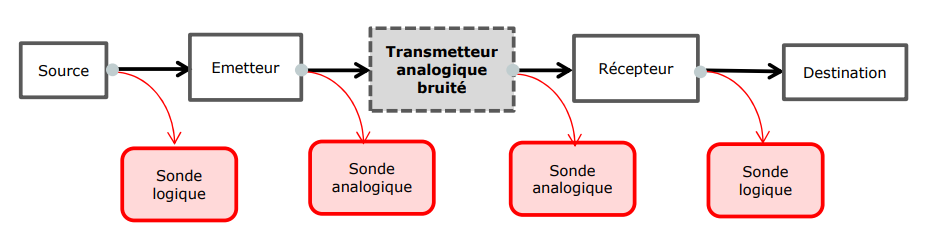
\includegraphics[width=1\textwidth]{image 21.png}
\caption{\label{fig:image21}Schéma de l'itération n°4.}
\end{figure}

Ci-dessous le schéma correspondant à l'ajout du bruit "réel" pour cette itération.

\begin{figure}[H]
\centering
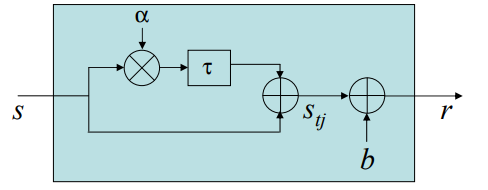
\includegraphics[width=1\textwidth]{image 22.png}
\caption{\label{fig:image22}Schéma d'ajout de bruit de l'itération n°4.}
\end{figure}

\subsubsection{correction des itérations précédentes}

Nous avons optimisé notre code précédent, cela nous permet de gagner du temps de calcul lorsque nous simulons un nombre important d'échantillons.  

\subsection{Organisation}

 Nous allons devoir créer de nouveaux éléments par rapport au code de l'itération précédente. Ces modifications devrons nous aider à lancer le programme tout en prenant en compte la génération de ce nouveau type de bruit que nous retrouvons dans les canaux de transmission suite aux différentes perturbations. Nous ne devrions pas avoir d'erreurs sur notre code cependant, nous devrions pouvoir observer les conséquences de l'ajout du bruit "réel" sur le signal. Nous pourrions voir tout cela grâce à la simulation des signaux mais également à de graphes. Pour vérifier le bon fonctionnement de notre code nous nous appuierons donc sur ces dernières. Dans le but d'effectuer ces modifications, nous avons amélioré le diagramme de Gant que nous avions utilisé lors de nos précédentes itérations. Voici à quoi il ressemble pour cette itération.
 
\subsection{Procédure de développement}

Développer un code lisible est indispensable pour avoir un programme efficace et facile à maintenir. Nous avons donc décidé de faire hériter notre classe $TransmetteurBruiteMultiTrajets$ par $TransmetteurBruiteAnalogique$. Cela nous permet d'ajouter du bruit à notre signal avec multi-trajet facilement sans avoir à connecter un transmetteur bruité avec un transmetteur multi-trajet. On évite alors quelques copies et nous gagnons alors en performances. Le plus important est de fragmenter le code de sorte à avoir une méthode par fonctionnalité. Cela nous permet de mieux nous organiser et de mieux travailler en collaboration sur le même code. A ce stade du projet, l'utilisation de git nous à permis également de diviser les taches en travaillant sur une branche par fonctionnalité. Nous pouvons donc chacun de notre coté altérer le code sans causer de problème aux autres.

\begin{figure}[H]
\centering
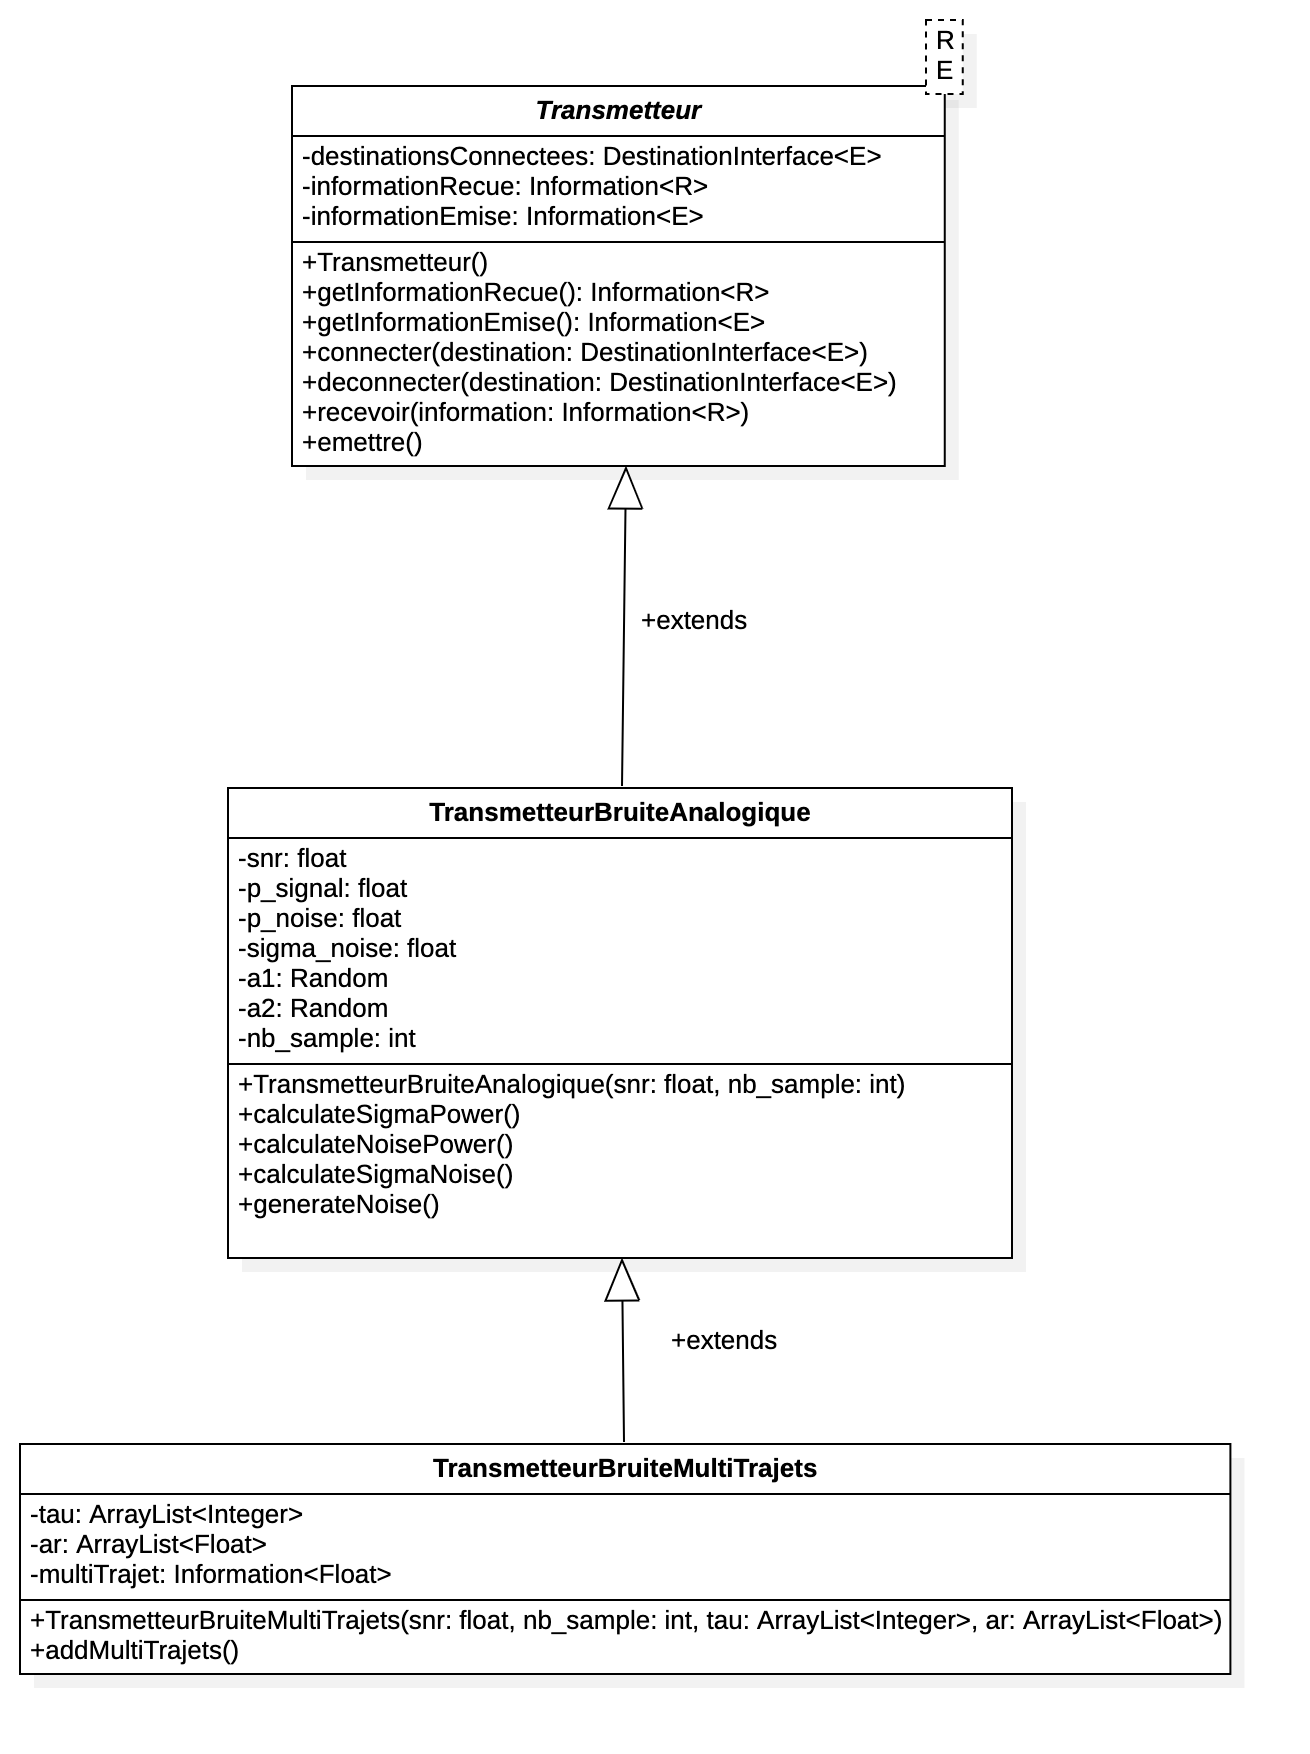
\includegraphics[width=\textwidth]{img/transm_multiTrajets.png}
\caption{\label{fig:image23}Diagramme de classes de l'implémentation du multi-trajet.}
\end{figure}

\pagebreak

\subsection{Trajets multiples}

L'objectif de cette itération est de voir l'impact de trois facteurs différents sur le récepteur. 

\subsubsection{impact des trajets multiples}

Nous allons nous intéresser maintenant à l'impact des trajets multiples. Pour ce faire nous allons effectuer deux simulations où le retard sera de 0 et les trajets auront la même amplitude. Le message émis est le même.

\begin{figure}[H]
\centering
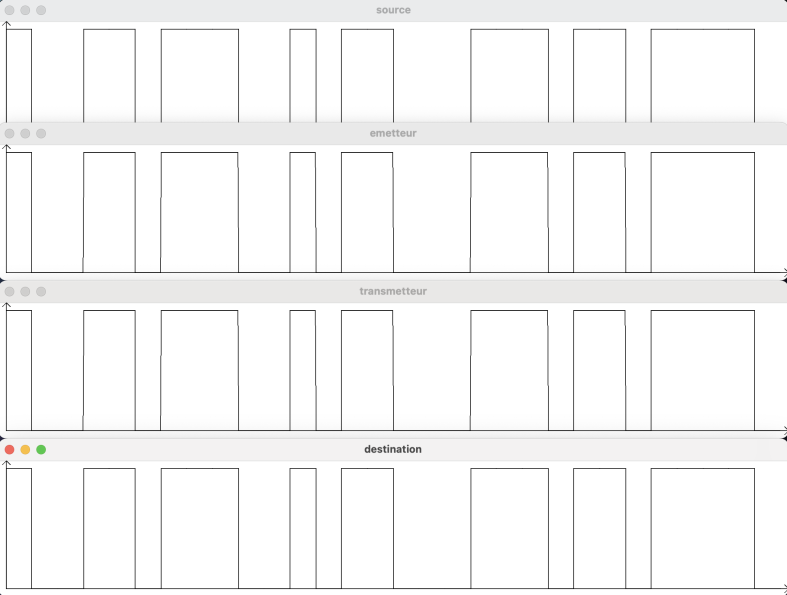
\includegraphics[width=\textwidth]{img/nulledecalage.png}
\caption{\label{fig:image25}Simulation avec 2 trajets multiples avec amplitude à 0}
\end{figure}

\begin{figure}[H]
\centering
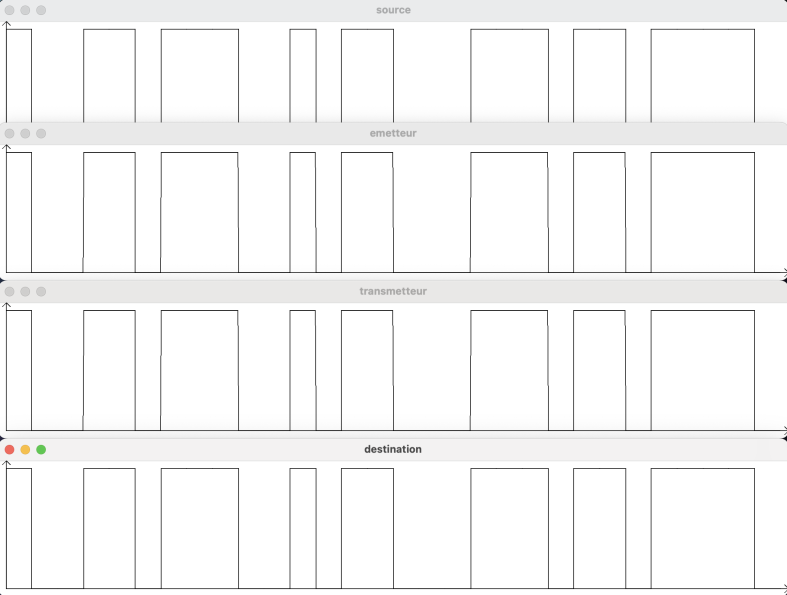
\includegraphics[width=\textwidth]{img/nulledecalage.png}
\caption{\label{fig:image25}Simulation avec 5 trajets multiples avec amplitude à 0}
\end{figure}

On constate que le TEB est de 0 dans les deux cas. Le multi trajet n'a pas d'impact s'il n'y a pas de retard ou de changement d'amplitude.


\subsubsection{impact du retard et de l'atténuation}
Dans cette partie, nous allons étudier l'impact du retard et de l'atténuation lors de trajets multiples. Nos signaux vont être reçu par le récepteur avec un décalage plus ou moins important. Tout d'abord voici la simulation avec deux trajets (le trajet direct et 1 trajet retardé) ayant la même amplitude et un retard de 20 échantillons.

(-s  -seed  99  -mess  30  -form  NRZ  -nbEch  100  -ampl  0  2  -snrpb  1000  -ti  20 0.9)

\begin{figure}[H]
\centering
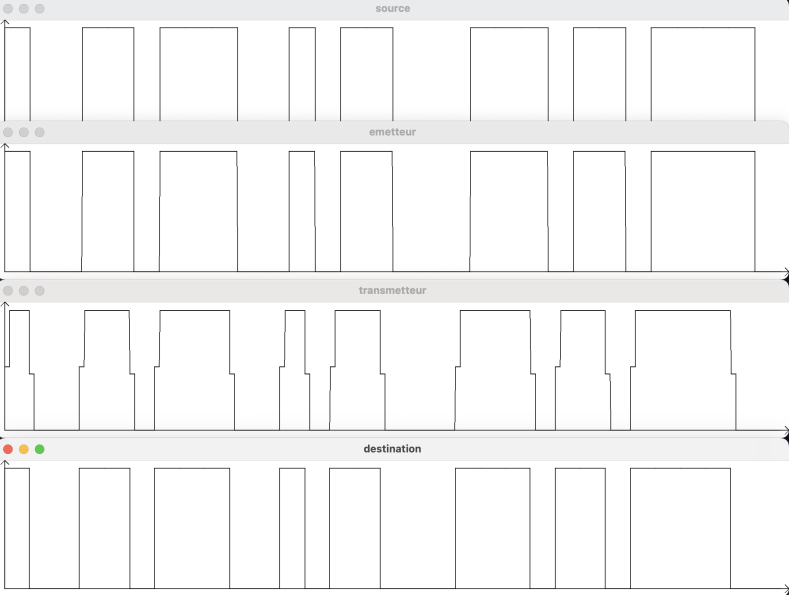
\includegraphics[width=\textwidth]{img/peuretard.png}
\caption{\label{fig:image25}Simulation avec 2 trajets multiples et un léger retard}
\end{figure}

On observe que le signal en sortie d'émetteur et de récepteur est le même. Le peu de retard n'impacte pas nos le décodage en réception. On effectue une nouvelle simulation mais cette fois ci, le deuxième signal aura un décalage de 80 échantillons.

(-s  -seed  99  -mess  30  -form  NRZ  -nbEch  100  -ampl  0  2  -snrpb  1000  -ti  80 0.9)

\begin{figure}[H]
\centering
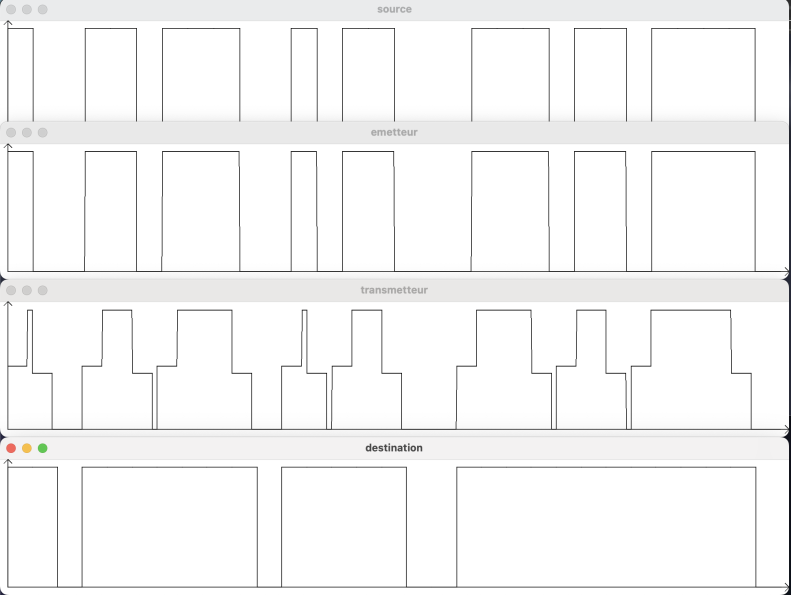
\includegraphics[width=\textwidth]{img/beaudecalage.png}
\caption{\label{fig:image25}Simulation avec 2 trajets multiples et un retard d'un demi symbole}
\end{figure}

Cette fois-ci, on n'obtient plus le même signal qu'à l'origine. Cela conclut le fait que le retard est un facteur important à prendre en compte lors de transmission multi-trajets. Une mauvaise gestion de ce dernier peut rendre notre système de transmission inopérant. 
Pour finir, nous allons étudier l'impact des amplitudes des multi-trajets. Pour ce faire, nous allons reprendre le multi-trajet précédents (même retard) mais nous allons baisser l'amplitude des signaux retardés de  80\%. 

( -s  -seed  99  -mess  30  -form  NRZ  -nbEch  100  -ampl  0  2  -snrpb  1000  -ti  100  0.1  100  0.1)

\begin{figure}[H]
\centering
\includegraphics[width=\textwidth]{img/atténuation.png}
\caption{\label{fig:image25}Simulation avec 2 trajets multiples retardé avec une amplitude plus importante pour le signal non décalé}
\end{figure}

On remarque que les signaux retardés n'interfèrent plus avec notre signal initial. Notre décodeur retrouve le même signal qu'à l'émission. Ainsi, si les signaux décalés ont une amplitude beaucoup plus faible que le signal non retardé, il n'y aura pas d'impact à la réception.
\subsubsection{Performances du code}

Dans une optique de performances plus rapides, nous avons réalisé un changement majeur dans le code de la classe $Information$. Cette modification consiste au passage des $LinkedList$ vers des $ArrayList$. Cette mise à jour du code est significative particulièrement a cause de notre façon de traiter les informations. Nous écrivons beaucoup dans de nouvelles listes sans particulièrement les modifier. Les LinkedList étant performantes pour la modification de données dans le tableau, cela ne nous est pas utile dans notre cas d'usage. Les ArrayList quant à elles sont très performantes mais beaucoup plus lentes pour la modification d'informations à l'intérieur de la liste. Ces opérations n'étant rarement voir jamais réalisés il alors logique pour notre groupe de changer de type de liste. La classe $Information$ nous facilite la vie car, en effet cela ne nous demande que quelques lignes à modifier dans le programme.

\subsection{Conclusion}

Pour conclure cette itération, nous avons pu étudier sur les multi-trajets. Grâce aux simulations, nous avons pu comprendre l'impact du retard et des atténuations sur le récepteur. Cela nous a permis de comprendre l'importance de ces paramètres et la nécessité d'avoir des correcteurs à ceux-ci.
Dans l'itération suivante, nous allons implémenter un codage de canal afin de corriger les  éventuels erreurs à la réception. 
\pagebreak

%--/Paper--

\end{document}